\chapter{जीवित मिट्टी}\label{ch:b2:living-soil}

चार्ल्स डार्विन की अंतिम पुस्तक, जो उनकी मृत्यु से एक वर्ष पहले छपी,
केंचुओं के बारे में थी। उन्होंने 1842 में अपने घर के पास किसी खेत पर
चाक का कोई चिह्न रखा था और 1871 में उसे खोद निकाला: वह अठारह सेंटीमीटर
नीचे पड़ा था, उन ढेरियों से गड़ा जो वे कीड़े सतह पर लाए थे,
और वह भी ऐसी दर से जो उन्होंने मापी, तोली, और गुणा की --- यानी प्रति एकड़
प्रति वर्ष दस टन \omterm{def:b2:living-soil:soil}{मिट्टी} उनकी देहों से होकर गुज़रती, ताकि
``ऐसे किसी भी विस्तार पर की सारी सतही \omterm{def:b2:living-soil:soil}{मिट्टी} हर कुछ वर्षों में
कीड़ों की देहों से गुज़र चुकी है, और फिर गुज़रेगी।''
दूसरे शब्दों में, \omterm{def:b2:living-soil:soil}{मिट्टी} कोई ऐसा आधार नहीं है जिस पर जीव
खड़े हों बल्कि कोई ऐसी चीज़ है जो जीव बनाते हैं। यह अध्याय
उसी बनाने के बारे में है: चट्टान \omterm{def:b2:living-soil:soil}{मिट्टी} कैसे बनती है और कितनी धीरे, उसमें कौन
रहता है और कितनी संख्या में, मरा हुआ पदार्थ कैसे खोला जाता है और
क्या बचता है, पौधों की जड़ें उसके लिए जो वे अकेले नहीं पा सकतीं कवकों तथा
जीवाणुओं से कैसे सौदा करती हैं, और जिस \omterm{def:b2:living-soil:soil}{मिट्टी} को बनने में
दस हज़ार वर्ष लगे वह कितनी तेज़ खोई जा सकती है।

\section{मिट्टी है क्या}

\begin{definition}[मिट्टी और उसके संस्तर]\label{def:b2:living-soil:soil}
\index{मिट्टी}\index{मिट्टी-संस्तर}\index{ह्यूमस}\index{अपक्षय}\index{मृदाजनन}
\emph{मिट्टी} अपक्षयित खनिज पदार्थ, कार्बनिक
पदार्थ, जल, वायु तथा जीवों की वह परत है जो स्थल को ढकती है और
पौधों को सँभालती है: उसके आयतन का लगभग आधा छिद्र हैं, जो बदलते अनुपात में
जल या वायु से भरे हैं, और वह ठोस आधा खनिज कण हैं ---
बालू (\qtyrange{0.05}{2}{mm}), गाद (\qtyrange{2}{50}{\micro m}) तथा
मृत्तिका (\qty{2}{\micro m} से नीचे), जिनके अनुपात उसका
\emph{गठन} देते हैं --- और कुछ प्रतिशत कार्बनिक पदार्थ जो
उसके अधिकांश गुण बाँधता है। किसी मिट्टी-परिच्छेदिका में
\emph{संस्तर} दिखते हैं: सतह पर कूड़े तथा अधकचरे क्षयित
कार्बनिक पदार्थ का \emph{O} संस्तर; \emph{ह्यूमस} से मिली खनिज
मिट्टी का गहरा \emph{A} संस्तर, यानी अपघटन का वह स्थिर, गहरा, कोलाइडी अवशेष;
नीचे \emph{B} संस्तर, जिसमें मृत्तिका,
लोहा तथा घुला पदार्थ बह आते हैं और जहाँ वे जमा होते हैं;
अपक्षयित जनक-चट्टान का \emph{C} संस्तर; और वह आधार-चट्टान। कोई
मिट्टी पाँच कारकों से बनती है (\emph{मृदाजनन}) --- जनक
पदार्थ, जलवायु, जीव, स्थलाकृति तथा समय --- और वह
धीरे बनती है: अपक्षय वर्ष भर में \qty{0.1}{mm} की कोटि की
मिट्टी बनाता है, इसलिए मीटर भर मिट्टी दस हज़ार वर्ष का काम है।
\end{definition}

\begin{omfigure}
\begin{tikzpicture}[every node/.style={font=\scriptsize}]
  \fill[brown!25!black!60] (0,5.4) rectangle (4,5.8); \node[right] at (4.2,5.6) {O: कूड़ा, काई, अधकचरा क्षयित पदार्थ (कुछ cm)};
  \fill[brown!60!black] (0,4.2) rectangle (4,5.4); \node[right, align=left] at (4.2,4.8) {A: ह्यूमस से मिली खनिज मिट्टी, गहरी, कणिका-संरचना वाली;\\ अधिकांश जड़ें, अधिकांश जीव (\qtyrange{10}{30}{cm})};
  \fill[brown!70!orange!80] (0,2.4) rectangle (4,4.2); \node[right, align=left] at (4.2,3.3) {B: ऊपर से बह आई मृत्तिका, लोहे के ऑक्साइड, कार्बोनेट\\ का जमाव; थोड़ी जड़ें (\qtyrange{30}{100}{cm})};
  \fill[gray!50!brown!60] (0,1.0) rectangle (4,2.4); \node[right, align=left] at (4.2,1.7) {C: अपक्षयित जनक-चट्टान, महीन आधात्री में टुकड़े};
  \fill[gray!70] (0,0) rectangle (4,1.0); \node[right] at (4.2,0.5) {R: आधार-चट्टान};
  \foreach \x in {0.4,1.3,2.5,3.4} \draw[brown!30!black, thick] (\x,5.4) .. controls (\x+0.2,4.8) and (\x-0.2,4.4) .. (\x+0.1,3.6);
  \foreach \x/\y in {0.7/3.0, 2.0/2.7, 3.2/3.3, 1.5/1.6, 3.0/1.9} \fill[gray!80] (\x,\y) ellipse (0.18 and 0.1);
  \draw[<->, thick] (-0.4,5.8) -- (-0.4,0) node[midway, left, rotate=90, anchor=south] {लगभग एक से दो मीटर};
\end{tikzpicture}

{\small कोई मिट्टी-परिच्छेदिका। कार्बनिक पदार्थ ऊपर से घुसता है और
उतरते-उतरते खपा दिया जाता है; खनिज पदार्थ तली पर छोड़ा जाता है
और जड़ों तथा प्राणियों से ऊपर चलाया जाता है; और घुला पदार्थ उस जल के साथ
नीचे चलता है तथा B संस्तर में पकड़ लिया जाता है।}
\end{omfigure}

\begin{proposition}[मृत्तिका और ह्यूमस क्यों मायने रखते हैं]\label{prop:b2:living-soil:cec}
\index{धनायन विनिमय क्षमता}\index{मृत्तिका}\index{मिट्टी-संरचना}\index{क्षेत्र-धारिता}
मृत्तिका-कण तथा \omterm{def:b2:living-soil:soil}{ह्यूमस} अपनी सतहों पर ऋण आवेश ढोते हैं
और, स्थिरवैद्युत आकर्षण से, विनिमेय धनायनों का कोई \omterm{def:b2:biogeochemical-cycles:reservoir}{भंडार} थामे रहते हैं
--- $\mathrm{Ca^{2+}}$, $\mathrm{Mg^{2+}}$, $\mathrm{K^{+}}$, $\mathrm{NH_4^{+}}$ --- जिन पर
पौधों की जड़ें उनके बदले $\mathrm{H^{+}}$ देकर हाथ डालती हैं। यह
\emph{\omterm{prop:b2:living-soil:cec}{धनायन विनिमय क्षमता}} \omterm{def:b2:living-soil:soil}{मिट्टी} का पोषक-बैंक है; किसी बालू में
लगभग कुछ भी नहीं (प्रति किलोग्राम कुछ सेंटीमोल आवेश), \omterm{def:b2:living-soil:soil}{ह्यूमस} से भरी किसी
मृत्तिका-दुमट में उससे पचास गुना, और दोनों की उर्वरता
उसी के अनुसार भिन्न है। वही सतहें जल भी थामती हैं: कोई बलुई \omterm{def:b2:living-soil:soil}{मिट्टी}
दिन भर के भीतर बहकर अपने आयतन के दसवें भाग की \emph{क्षेत्र-धारिता} तक
आ जाती है, कोई दुमट एक तिहाई थामती है, और वह अंतर ही वह है जो किसी फ़सल के पास
वर्षाओं के बीच होता है। और \omterm{def:b2:living-soil:soil}{ह्यूमस}, कवक-तंतुओं,
जड़-स्रावों तथा कीड़ों के श्लेष्म के साथ, खनिज कणों को
\emph{समुच्चयों} में जोड़ देता है, यानी वह कणिका-संरचना जिसके छिद्र वायु, जल
तथा जड़ों को गुज़रने देते हैं --- यानी वह गुण जो किसी \omterm{def:b2:living-soil:soil}{मिट्टी} को किसी
अवसाद से अलग करता है और जिसे हल तथा संपीडन सबसे पहले नष्ट करते हैं।
\end{proposition}

\section{वहाँ कौन रहता है}

\begin{proposition}[मिट्टी का समुदाय]\label{prop:b2:living-soil:community}
\index{मिट्टी का आहार-जाल}\index{अपरदभक्षी}\index{केंचुआ}\index{मिट्टी-जैवभार}
उर्वर ऊपरी \omterm{def:b2:living-soil:soil}{मिट्टी} का एक ग्राम कोई दस हज़ार जातियों की $10^{9}$
जीवाणु-कोशिकाएँ, सौ मीटर कवक-तंतु, $10^{4}$
\omterm{def:b2:unicellular-diversity:protist}{प्रोटिस्ट}, कुछ दर्जन सूत्रकृमि तथा मुट्ठी भर माइट और
संतुलक थामे है; और कोई वर्ग मीटर कुछ सौ केंचुए थामे है तथा,
दिखने वाले प्राणियों के नीचे, प्रति हेक्टेयर कई टन का कोई जीवित द्रव्यमान ---
यानी उतना ही जितने मवेशी वही हेक्टेयर सँभाल सकता है।
वह समुदाय कोई \emph{अपरद आहार-जाल} है: जीवाणु तथा कवक
(यानी \emph{अपघटक}) मरा पदार्थ खाते हैं और \omterm{def:b2:unicellular-diversity:protist}{प्रोटिस्टों}
तथा सूत्रकृमियों (यानी सूक्ष्मजीव-चरने वालों) से खाए जाते हैं, जिन्हें माइट तथा
परभक्षी सूत्रकृमि खाते हैं, जो कनखजूरों तथा भृंगों को पोसते हैं; और
\emph{अपरदभक्षी} --- केंचुए, सहस्रपाद, वुडलाइस, दीमक,
संतुलक --- वह कूड़ा स्वयं उस पर के सूक्ष्मजीवों समेत खाते हैं,
और उसे हज़ार गुना तोड़कर उस सतह को गुणा कर देते हैं जिस पर
सूक्ष्मजीव हमला करते हैं। वे चरने वाले अपनी संख्या से आगे मायने रखते हैं: जीवाणु खाकर
वे जीवाणु-कोशिकाओं में बंद नाइट्रोजन अमोनियम के रूप में छोड़ देते हैं,
और \omterm{def:b2:unicellular-diversity:protist}{प्रोटिस्टों} तथा सूत्रकृमियों वाली कोई \omterm{def:b2:living-soil:soil}{मिट्टी} अकेले जीवाणुओं वाली किसी से
तेज़ नाइट्रोजन खनिजित करती है। केंचुए वे
\emph{पारितंत्र-अभियंता} हैं: उनकी बिल \omterm{def:b2:living-soil:soil}{मिट्टी} के
वृहत्-छिद्र हैं, उनकी ढेरियाँ सबसे समृद्ध समुच्चय हैं, और किसी
घास-भूमि के कीड़े हर वर्ष प्रति हेक्टेयर कुछ टन \omterm{def:b2:living-soil:soil}{मिट्टी} अपनी आँतों से
गुज़ार देते हैं, जैसा डार्विन ने मापा।
\end{proposition}

\begin{omfigure}
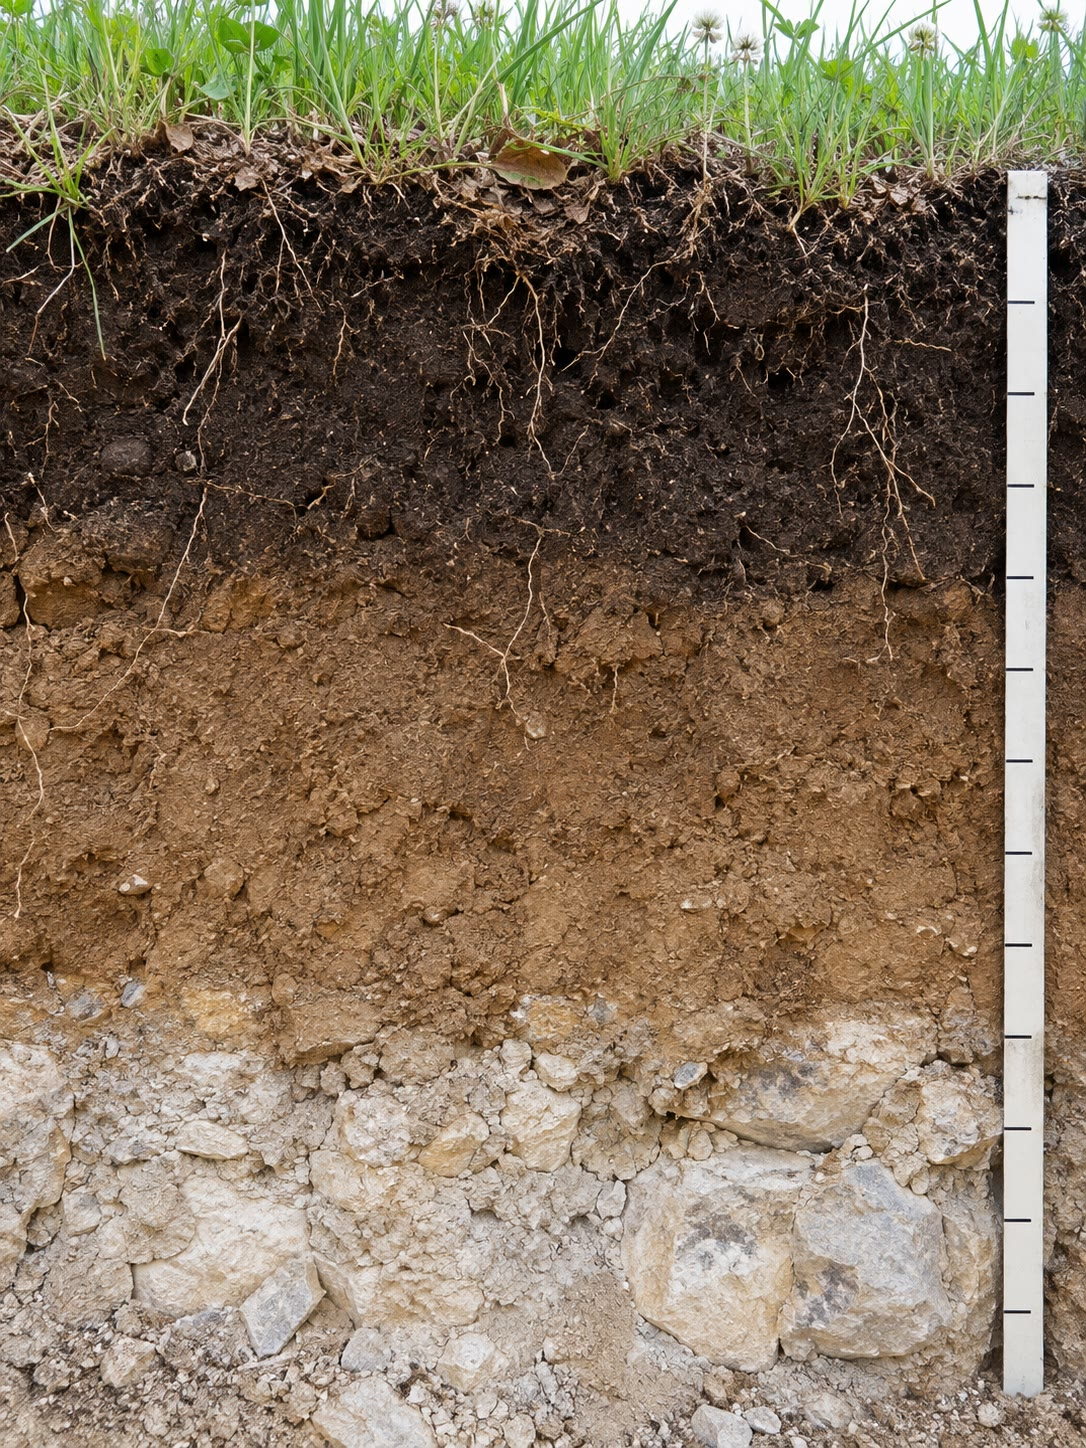
\includegraphics[width=0.21\linewidth]{images/book4/ai/b4-26-soil-profile.jpg}\hspace{0.025\linewidth}
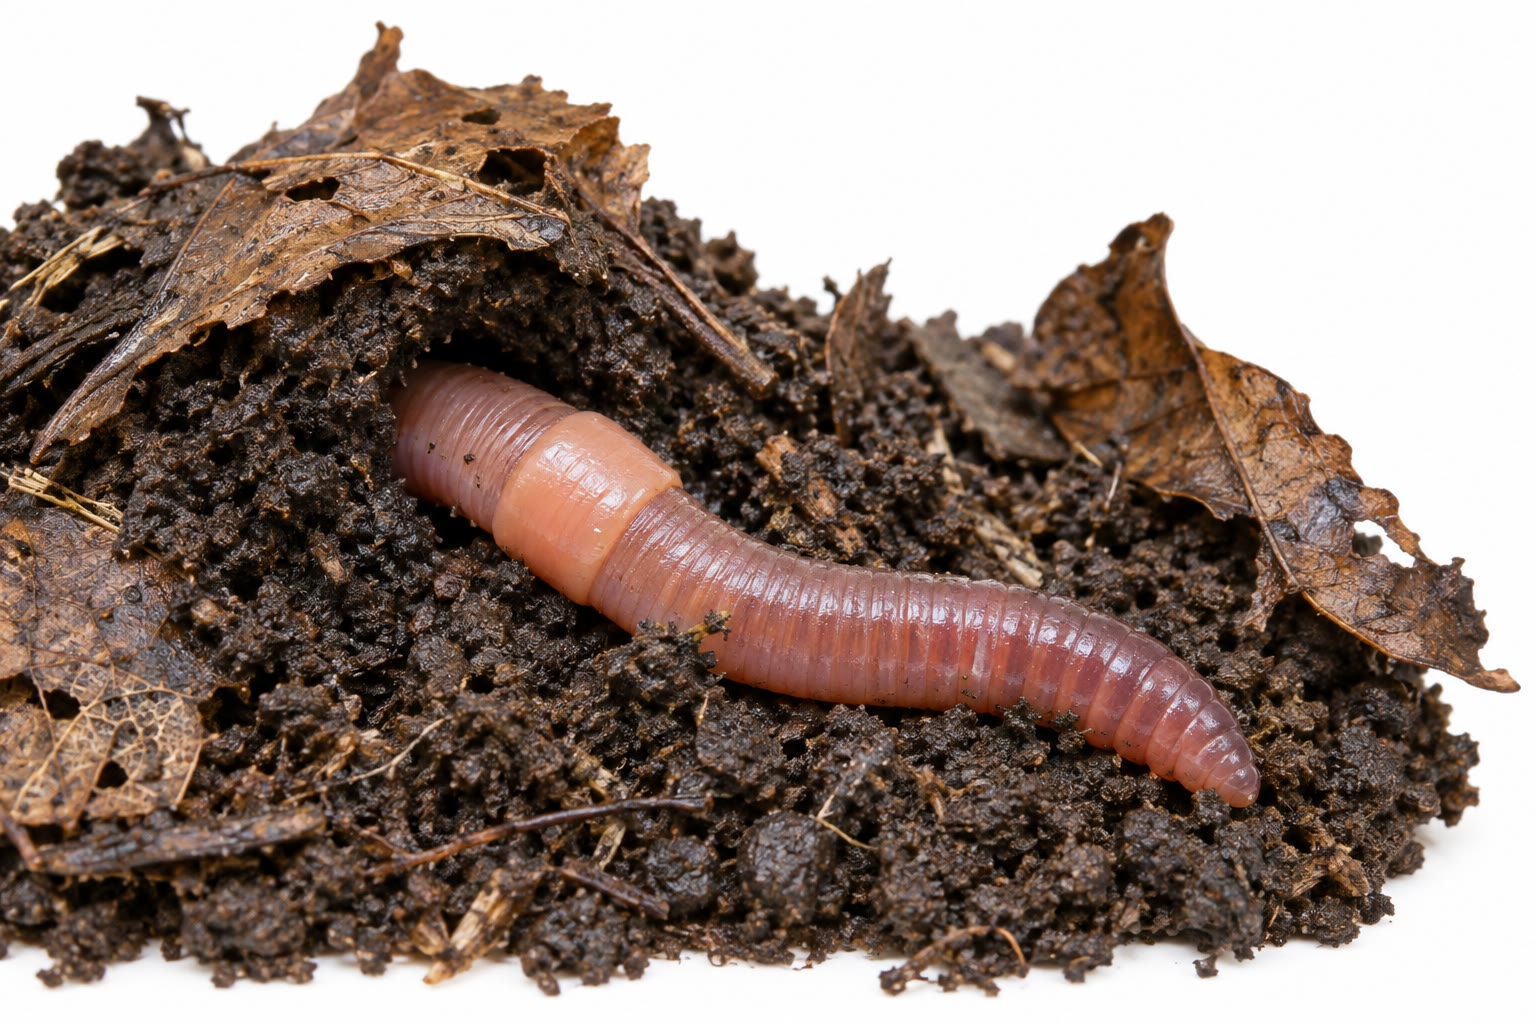
\includegraphics[width=0.42\linewidth]{images/book4/ai/b4-26-earthworm.jpg}\hspace{0.025\linewidth}
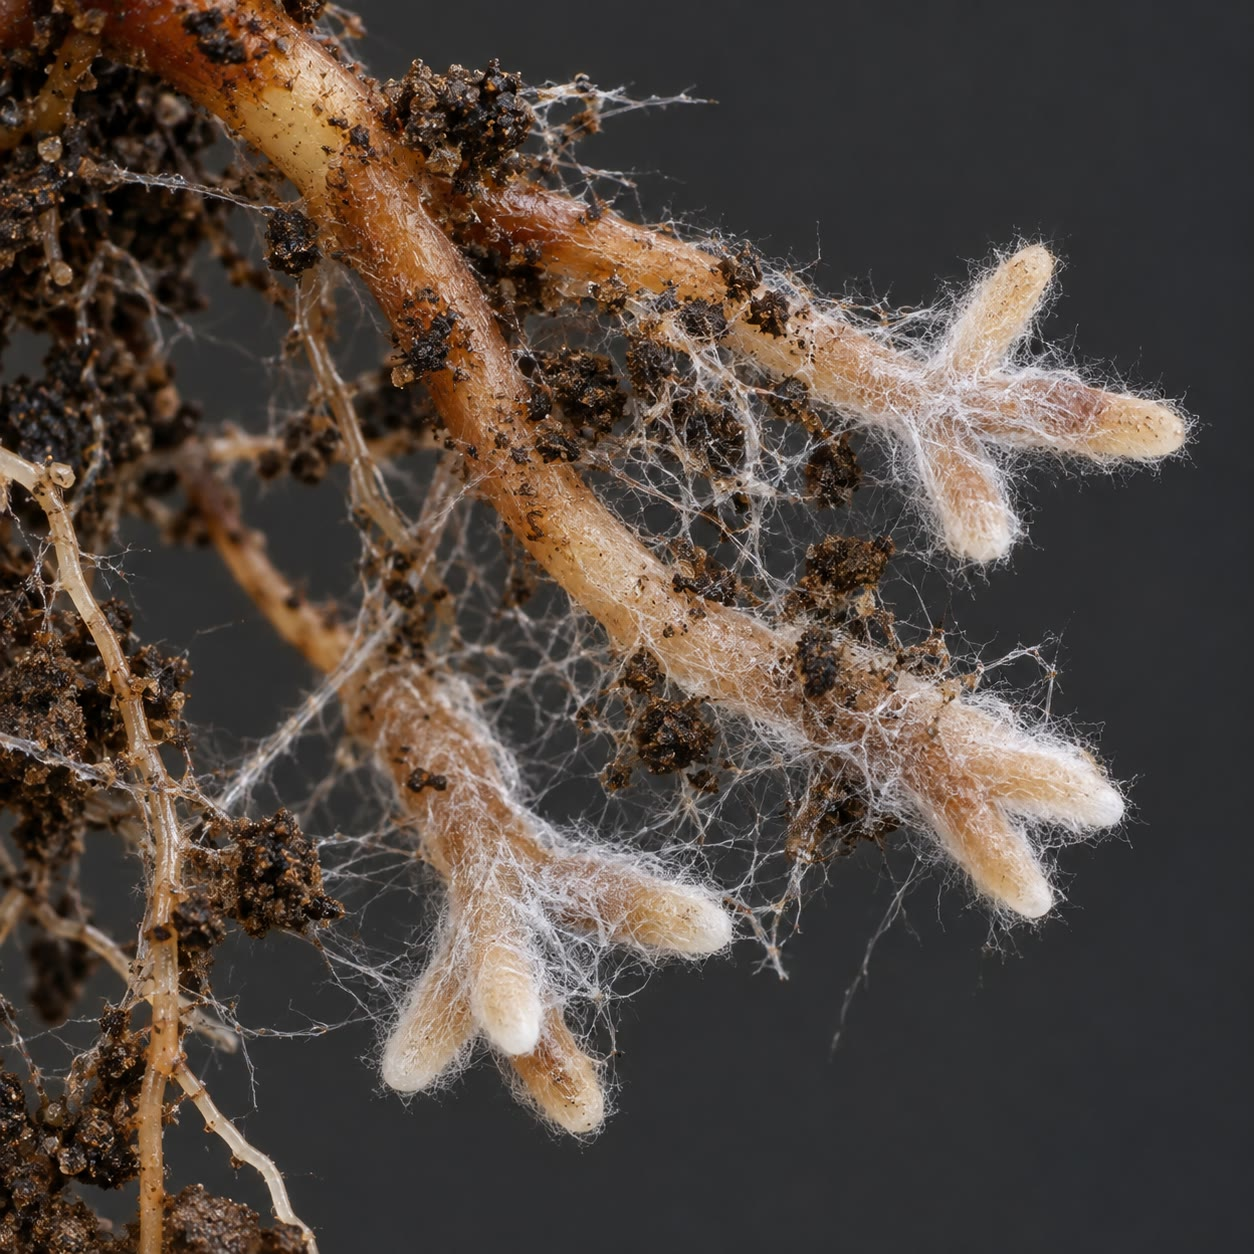
\includegraphics[width=0.28\linewidth]{images/book4/ai/b4-26-mycorrhiza.jpg}

{\small वह \omterm{def:b2:living-soil:soil}{मिट्टी} और उसके दो निर्माता। बाएँ: किसी कटे
किनारे में कोई परिच्छेदिका, गहरी ऊपरी \omterm{def:b2:living-soil:soil}{मिट्टी} जो नीचे पीली अपक्षयित चट्टान में ढलती है। बीच में: अपनी बिल में
कोई केंचुआ। दाएँ: अपने बाह्यकवकमूली
ग़िलाफ़ तथा उन तंतुओं समेत कोई जड़ जो उसे \omterm{def:b2:living-soil:soil}{मिट्टी} में फैला देते हैं।}
\end{omfigure}

\section{अपघटन}

\begin{theorem}[कूड़े का क्षय और कार्बन-से-नाइट्रोजन अनुपात]\label{thm:b2:living-soil:decay}
\index{अपघटन}\index{कूड़े का क्षय}\index{C:N अनुपात}\index{खनिजीकरण}\index{स्थिरीकरण (नाइट्रोजन)}
कूड़ा जो बचा हो उसके समानुपाती दर से अपघटित होता है,
$\mathrm{d}L/\mathrm{d}t = -kL$, इसलिए $L = L_0 e^{-kt}$, जिसमें कोई
\emph{क्षय नियतांक} $k$ है, जो किसी समशीतोष्ण वन में घास तथा
पर्णपाती पत्तियों के लिए लगभग 1 प्रति वर्ष है, शंकुधारी सूइयों के लिए $0.3$,
गीले उष्णकटिबंध में कई प्रति वर्ष और टुंड्रा में $0.05$;
और प्रति वर्ष कोई अचल निवेश $I$ $I/k$ की कोई कूड़ा-परत बना देता है। क्षय
ताप, नमी, और उस कूड़े की \emph{गुणता} से नियंत्रित होता है:
यानी नाइट्रोजन-मात्रा, लिग्निन-मात्रा, और
कार्बन का नाइट्रोजन से अनुपात। सूक्ष्मजीवों का $\mathrm{C:N} \approx 8$ है और वे
जो कार्बन खाएँ उसका लगभग \qty{40}{\%} रखते हैं, इसलिए उन्हें भोजन के हर
$8/0.4 = 20$ कार्बनों के लिए एक नाइट्रोजन चाहिए: लगभग 25 से नीचे $\mathrm{C:N}$ वाला
कूड़ा क्षय होते समय अमोनियम छोड़ता है
(\emph{खनिजीकरण}), जबकि उससे ऊपर वाला कूड़ा --- 80 पर पुआल,
400 पर काठ --- सूक्ष्मजीवों से \omterm{def:b2:living-soil:soil}{मिट्टी} की नाइट्रोजन लिवा लेता है
(\emph{स्थिरीकरण}), और पौधों को तब तक भूखा रखता है जब तक वह कार्बन
श्वसित न हो जाए और वह अनुपात न गिर जाए। इसीलिए हल से जोता गया ताज़ा
पुआल किसी फ़सल को दबा देता है, इसीलिए शिंबी-अवशेष उसे पोसता है,
और इसीलिए किसी कंपोस्ट-ढेर को दोनों चाहिए।
\end{theorem}
\begin{proof}
उस अनुपात के लिए: जो सूक्ष्मजीव प्रति नाइट्रोजन $c$ कार्बन वाला कूड़ा खाएँ
वे $0.4c$ कार्बन स्वांगीकृत करते हैं और, $\mathrm{C:N} = 8$ पर
जैवभार बनाने को, उन्हें $0.4c/8 = c/20$ नाइट्रोजन चाहिए; और वह कूड़ा
1 देता है। यदि $c < 20$ हो तो बचाने भर नाइट्रोजन है, जो अमोनियम के रूप में
छोड़ी जाती है; और यदि $c > 20$ हो तो कोई घाटा है जो \omterm{def:b2:living-soil:soil}{मिट्टी} से लिया जाता है।
व्यवहार में देहली 25 0.4 से कुछ नीची किसी
धारण-दक्षता को दर्शाती है। उस कूड़ा-परत के लिए: $\mathrm{d}L/\mathrm{d}t = I - kL$
की \omterm{def:b2:biogeochemical-cycles:reservoir}{स्थायी अवस्था} $I/k$ है, जिस तक काल-नियतांक $1/k$ से पहुँचा जाता है; और
कूड़े का \omterm{def:b2:biogeochemical-cycles:reservoir}{निवास-काल} $1/k$ है, यानी किसी बीच-वन में एक वर्ष और
टुंड्रा में बीस।
\end{proof}
\begin{proof}[प्रमाण-सामग्री]
कूड़ा-थैली प्रयोगों ने --- जाली की थैलियों में पत्तियों के ज्ञात द्रव्यमान,
गाड़े गए और अंतरालों पर तोले गए --- हर जीवोम भर वह चरघातांकी नियम तथा
उसके नियतांक दिए (ओल्सन, 1963), और भिन्न जाली-आकारों से दिखाया
कि \omterm{def:b2:living-soil:soil}{मिट्टी} के प्राणियों को हटाने से वह दर आधी हो जाती है:
यानी रसायन सूक्ष्मजीव करते हैं पर चाल प्राणी बाँधते हैं।
किसी महाद्वीप भर, वही पत्ती जॉर्जिया में एक वर्ष में और
अलास्का में आठ में क्षय होती है, यानी वास्तविक वाष्पोत्सर्जन-वाष्पन के,
जो गरमाहट तथा जल का गुणनफल है, समानुपात में।
\end{proof}

\begin{omfigure}
\begin{tikzpicture}
\begin{axis}[
  width=0.72\linewidth, height=5.6cm,
  axis x line=bottom, axis y line=left,
  xmin=0, xmax=6, ymin=0, ymax=105,
  xlabel={वर्ष}, ylabel={बचा कूड़ा-द्रव्यमान (\%)},
  xlabel style={font=\small, at={(axis description cs:0.5,-0.13)}, anchor=north},
  ylabel style={font=\small},
  tick label style={font=\small},
  legend style={font=\scriptsize, at={(0.5,-0.3)}, anchor=north, draw=none, legend columns=2},
  clip=false,
]
\addplot[very thick, omDef, domain=0:6, samples=60] {100*exp(-2*x)};
\addlegendentry{उष्णकटिबंधीय वन की पत्ती, $k = 2$}
\addplot[very thick, omThm, domain=0:6, samples=60] {100*exp(-1*x)};
\addlegendentry{बीच की पत्ती, $k = 1$}
\addplot[very thick, omProp, domain=0:6, samples=60] {100*exp(-0.3*x)};
\addlegendentry{स्प्रूस की सूई, $k = 0.3$}
\addplot[very thick, gray, domain=0:6, samples=60] {100*exp(-0.05*x)};
\addlegendentry{टुंड्रा की काई, $k = 0.05$}
\end{axis}
\end{tikzpicture}

{\small कूड़े का चरघातांकी क्षय। किसी बीच-पत्ती का आधा आठ महीनों में
चला जाता है; किसी टुंड्रा-काई का आधा चौदह वर्षों में; और वह
अवशेष जिसे न सूक्ष्मजीव न प्राणी पूरा कर सकें \omterm{def:b2:living-soil:soil}{ह्यूमस} बन जाता है।}
\end{omfigure}

\begin{proposition}[ह्यूमस और मिट्टी का कार्बन-कोष]\label{prop:b2:living-soil:humus}
\index{ह्यूमस}\index{मिट्टी का कार्बनिक कार्बन}\index{मिट्टी-श्वसन}
कूड़े के कार्बन का कुछ प्रतिशत पूरे ऑक्सीकरण से बच जाता है
और \emph{\omterm{def:b2:living-soil:soil}{ह्यूमस}} बन जाता है: यानी सूक्ष्मजीवी अवशेषों, बदले हुए लिग्निन तथा
पादप यौगिकों का कोई गहरा, अक्रिस्टलीय मिश्रण, जो मृत्तिका तथा
लोहे से बँधा और समुच्चयों में जकड़ा है, और जो दशकों से सहस्राब्दियों के \omterm{def:b2:biogeochemical-cycles:reservoir}{निवास-कालों} से
क्षय होता है। \omterm{def:b2:living-soil:soil}{ह्यूमस} ही वह है जहाँ \omterm{def:b2:living-soil:soil}{मिट्टी} की उर्वरता बसती है
--- यानी उसकी अधिकांश नाइट्रोजन तथा धनायन-विनिमय, उसका आधा जल-धारण ---
और वह स्थल पर कार्बनिक कार्बन का सबसे बड़ा कोष है,
यानी ऊपर के मीटर में \qty{1700}{GtC}, जो वायुमंडल से दुगुना है। उसका
संतुलन निवेश घटा क्षय है, $\mathrm{d}H/\mathrm{d}t = I_h - k_hH$:
$k_h \approx 0.02$ प्रति वर्ष के साथ कोई \omterm{def:b2:living-soil:soil}{मिट्टी} पचास वर्षों का निवेश थामे है,
और कोई भी परिवर्तन --- जोतना, जो उन समुच्चयों को तोड़ता है तथा
\omterm{def:b2:living-soil:soil}{ह्यूमस} को हवा देता है; किसी पीट का जल-निकास, जो ऑक्सीजन आने देता है;
तापन, जो $k_h$ चढ़ाता है --- ऐसी हानि के रूप में दिखता है जो दशकों तक
चलती रहती है। दुनिया की जोती गई मिट्टियाँ जब से पहली बार तोड़ी गईं तब से अपने
\omterm{def:b2:living-soil:soil}{ह्यूमस} का एक तिहाई से आधा खो चुकी हैं, यानी कोई
\qty{100}{GtC}, और \qty{3}{\celsius} का तापन बाक़ी के
क्षय को एक तिहाई चढ़ा देगा: मिट्टियाँ
\cref{ch:b2:global-change} के कार्बन बजट में सबसे बड़ी अनिश्चितता हैं।
\end{proposition}

\section{ज़मीन के नीचे साझेदारियाँ}

\begin{proposition}[कवकमूल और राइजोबिया]\label{prop:b2:living-soil:symbiosis}
\index{कवकमूल}\index{राइजोबियम}\index{मूल-ग्रंथिका}\index{नाइट्रोजनेज़}\index{लेग्हीमोग्लोबिन}
दस में से नौ पादप जातियों की जड़ें किसी \emph{कवकमूल} में कवकों से
बसाई गई हैं: वह पौधा शर्करा देता है (अपने प्रकाशसंश्लिष्ट का
दसवाँ से पाँचवाँ भाग) और वह कवक फ़ॉस्फ़ेट, नाइट्रोजन, जल तथा
जस्ता, जिन्हें उसके तंतु, जो किसी जड़ से सौ गुना पतले हैं और
प्रति इकाई कार्बन उसकी लंबाई से सौ गुना फैलते हैं, \omterm{def:b2:living-soil:soil}{मिट्टी} के ऐसे आयतन से
इकट्ठा करते हैं जहाँ वह जड़ पहुँच नहीं सकती --- विशेषकर फ़ॉस्फ़ेट,
जो \omterm{def:b2:living-soil:soil}{मिट्टी} में इतना धीरे विसरित होता है कि कोई जड़
अपने मिलीमीटर भर पड़ोस को दिनों के भीतर चुका देती है।
\emph{अर्बुस्कुली} कवकमूल, जो पुरानी क़िस्म है, जड़-कोशिकाओं में घुसती है
और उन अर्बुस्कुलों में शाखित होती है जहाँ वह विनिमय होता है;
जबकि वन-वृक्षों की \emph{बाह्यकवकमूल} जड़-सिरे को ग़िलाफ़ पहनाती है और
उसकी कोशिकाओं के बीच बढ़ती है। शिंबियाँ और आगे जाती हैं: राइजोबिया,
जड़ के फ़्लेवोनॉइडों से खिंचकर, किसी मूल-रोम से घुसते हैं, और वह जड़
उनके चारों ओर कोई \emph{ग्रंथिका} बना देती है जिसमें वे जीवाणु,
\emph{बैक्टीरॉइड} के रूप में, नाइट्रोजनेज़ से नाइट्रोजन स्थिर करते हैं --- यानी ऐसा एंजाइम जो
ऑक्सीजन के प्रति इतना संवेदी है कि उस ग्रंथिका को
\emph{लेग्हीमोग्लोबिन} से लगभग अनॉक्सी रखना पड़ता है, यानी ऐसे हीमोग्लोबिन से जो वह पौधा बनाता है, जो
उस ग्रंथिका को उसका गुलाबी रंग देता है और बैक्टीरॉइडों तक ऑक्सीजन
ऐसी सांद्रता पर पहुँचाता है जो उस एंजाइम को ज़हर देने को बहुत नीची है। हर साझेदार
दूसरे की चौकसी करता है: कोई पौधा उन ग्रंथिकाओं की शर्करा काट देता है जो कुछ भी
स्थिर न करें, और जो कवक कम फ़ॉस्फ़ेट पहुँचाए उसे कम
कार्बन मिलता है।
\end{proposition}
\begin{proof}[प्रमाण-सामग्री]
कीयर्स तथा सहयोगियों ने (2011) किसी बँटी जड़-प्रणाली पर दो कवक-साझेदारों के साथ
कोई पौधा उगाया और फ़ॉस्फ़ेट केवल एक ओर दिया:
उस पौधे ने उस कवक को अधिक कार्बन बाँटा जिसने अधिक
फ़ॉस्फ़ेट दिया, और उस कवक ने उस जड़ को अधिक फ़ॉस्फ़ेट बाँटा जिसने
अधिक कार्बन दिया --- यानी समस्थानिकों से मापे गए पारस्परिक पुरस्कार।
राइजोबिया के लिए, जिन ग्रंथिकाओं को प्रयोग से नाइट्रोजन नहीं दी गई (उस
वायु को आर्गन तथा ऑक्सीजन से बदलकर) उन्हें कम ऑक्सीजन मिली और वे
उसी पौधे की उन ग्रंथिकाओं से कम बढ़ीं जो स्थिर कर सकती थीं: यानी वह पौधा
ठगों पर प्रतिबंध लगाता है। नाइट्रोजन-15 अनुरेखण दिखाता है कि कोई क्लोवर--घास
का मैदान ऋतु भर के भीतर क्लोवर की स्थिर नाइट्रोजन का एक तिहाई उस
घास को दे देता है, \omterm{def:b2:living-soil:soil}{मिट्टी} से होकर तथा साझा
कवक-जालों से होकर।
\end{proof}

\begin{omfigure}
\begin{tikzpicture}[every node/.style={font=\scriptsize}, >=stealth]
  % root cross-section
  \fill[omThm!15] (0,0) circle (1.5); \draw[thick] (0,0) circle (1.5);
  \fill[omThm!30] (0,0) circle (0.5); \draw[thick] (0,0) circle (0.5);
  \node at (0,0) {रंभ};
  \node at (0,1.05) {वल्कुट};
  % arbuscules in cortex cells
  \foreach \a in {30,150,270} { \draw[omDef, thick] ({1.0*cos(\a)},{1.0*sin(\a)}) -- ++({0.25*cos(\a+60)},{0.25*sin(\a+60)}) -- ++({0.2*cos(\a-40)},{0.2*sin(\a-40)}); \draw[omDef, thick] ({1.0*cos(\a)},{1.0*sin(\a)}) -- ++({0.25*cos(\a-60)},{0.25*sin(\a-60)}); }
  % hyphae out
  \foreach \a in {20,80,150,210,340} { \draw[omDef, thick] ({1.5*cos(\a)},{1.5*sin(\a)}) .. controls ({2.2*cos(\a+10)},{2.2*sin(\a+10)}) .. ({2.7*cos(\a-5)},{2.7*sin(\a-5)}); }
  \draw[omDef, thick] ({1.5*cos(150)},{1.5*sin(150)}) -- ({1.0*cos(150)},{1.0*sin(150)});
  \node[omDef, anchor=west, align=left] at (2.9,1.4) {तंतु: \qty{3}{\micro m} चौड़े,\\ प्रति सेंटीमीटर जड़ मीटरों भर};
  \node[omDef, anchor=west] at (2.9,0.1) {किसी वल्कुट-कोशिका के भीतर अर्बुस्कुल};
  \draw[omDef] (2.85,0.1) -- (1.2,0.5);
  \node[anchor=north, align=center] at (0,-1.6) {जड़, \qty{0.3}{mm} चौड़ी};
  \draw[->, thick, omThm] (-1.2,-2.4) -- (1.2,-2.4) node[right] {कवक को शर्करा, प्रकाशसंश्लिष्ट का \qtyrange{10}{20}{\%}};
  \draw[<-, thick, omDef] (-1.2,-2.9) -- (1.2,-2.9) node[right] {पौधे को फ़ॉस्फ़ेट, अमोनियम, जल, जस्ता};
  % nodule
  \begin{scope}[xshift=9.3cm]
    \draw[thick, brown!60!black] (-0.3,2.4) -- (-0.1,-0.6);
    \draw[thick, brown!60!black] (-0.1,0.3) -- (1.6,0.1);
    \fill[pink!60!red!40] (1.5,0.2) circle (0.9); \draw[thick] (1.5,0.2) circle (0.9);
    \fill[pink!80!red!60] (1.5,0.2) circle (0.55);
    \foreach \p in {(1.3,0.3),(1.6,0.0),(1.5,0.45),(1.7,0.3),(1.35,0.05)} \fill[omDef!70!black] \p ellipse (0.08 and 0.05);
    \node[anchor=north, align=center] at (1.5,-0.8) {ग्रंथिका: पादप-कोशिकाओं में बैक्टीरॉइड,\\ लेग्हीमोग्लोबिन से गुलाबी;\\ ऑक्सीजन \qty{10}{nM} पर थमी, ताकि नाइट्रोजनेज़\\ चले और वे कोशिकाएँ फिर भी श्वसन करें};
    \node[anchor=south, align=center] at (-0.2,2.45) {शिंबी की जड़};
  \end{scope}
\end{tikzpicture}

{\small दो सौदे। बाएँ: कोई अर्बुस्कुली कवकमूल, जिसमें शर्करा बाहर
और फ़ॉस्फ़ेट भीतर वल्कुट-कोशिकाओं के भीतर के अर्बुस्कुलों से जाते हैं। दाएँ:
कोई शिंबी-ग्रंथिका, जहाँ उस पौधे का अपना हीमोग्लोबिन ऑक्सीजन
नाइट्रोजनेज़ भर नीची और श्वसन भर ऊँची रखता है।}
\end{omfigure}

\section{मिट्टी खोना}

\begin{proposition}[अपरदन, लवण और किसी मिट्टी का संतुलन]\label{prop:b2:living-soil:erosion}
\index{मिट्टी-अपरदन}\index{लवणीकरण}\index{मरुस्थलीकरण}
\omterm{def:b2:living-soil:soil}{मिट्टी} वर्ष भर में \qtyrange{0.05}{0.5}{mm} बनती है और, प्राकृतिक
वनस्पति के नीचे, लगभग उसी दर से अपरदित होती है। किसी ढलान पर नंगी जोती
ज़मीन वर्ष भर में जल तथा पवन को \qtyrange{1}{10}{mm} खोती है ---
यानी \qtyrange{10}{100}{t/ha} --- यानी बनने की दर से
दस से सौ गुना: यानी दस हज़ार वर्षों में बनी कोई \omterm{def:b2:living-soil:soil}{मिट्टी}
सदी भर में हट जाती है, और उसके साथ A संस्तर का \omterm{def:b2:living-soil:soil}{ह्यूमस} तथा पोषक,
यानी वही एक भाग जो मायने रखता है। आवरण-फ़सलें, सीढ़ियाँ, समोच्च जुताई
और बिना-जुताई खेती, जो अवशेष सतह पर तथा उन
समुच्चयों को अक्षत छोड़ती है, उस हानि को बनने की दर के पास वापस ले आती हैं।
शुष्क जलवायुओं में सिंचाई उलटी विफलता लाती है: जल
वाष्पित होता है और अपने लवण छोड़ जाता है, यानी ऐसे जल से प्रति हेक्टेयर प्रति वर्ष टन भर
जो थोड़ा ही लवणीय हो, जब तक मिट्टी-विलयन का परासरणी विभव
(\cref{ch:b2:plant-plasticity}) उससे नीचा न हो जाए जिसे वे
जड़ें पार कर सकें --- यानी \emph{लवणीकरण}, जिसने चार हज़ार वर्ष पहले
सुमेर के खेत सेवानिवृत्त कर दिए और अब सिंचित ज़मीन के
पाँचवें भाग को छूता है। किसी \omterm{def:b2:living-soil:soil}{मिट्टी} की दशा कोई बजट है: \omterm{def:b2:living-soil:soil}{ह्यूमस} भीतर बनाम
\omterm{def:b2:living-soil:soil}{ह्यूमस} बाहर, बनना बनाम अपरदन, लवण भीतर बनाम लवण
बाहर; और हर एक का कोई \omterm{def:b2:biogeochemical-cycles:reservoir}{निवास-काल} है, तथा हर एक, एक बार ऋण हो जाए, तो
उलटने में धीमा है।
\end{proposition}

\section{अभ्यास}

\begin{exercise}[$\star$]\label{exo:b2:living-soil:1}
सतह से नीचे तक किसी मिट्टी-परिच्छेदिका के संस्तर बताइए और कहिए
कि हर एक में क्या होता है।
\end{exercise}

\begin{exercise}[$\star$]\label{exo:b2:living-soil:2}
समझाइए कि \omterm{prop:b2:living-soil:cec}{धनायन विनिमय क्षमता} क्या है, किसी बलुई \omterm{def:b2:living-soil:soil}{मिट्टी} में वह
थोड़ी क्यों है, और जो किसान किसी अम्लीय \omterm{def:b2:living-soil:soil}{मिट्टी} में चूना डाले वह उसका क्या कर रहा है।
\end{exercise}

\begin{exercise}[$\star$]\label{exo:b2:living-soil:3}
अपघटकों से शीर्ष परभक्षियों तक \omterm{prop:b2:living-soil:community}{मिट्टी के आहार-जाल} के मुख्य समूह
गिनाइए, हर एक के लिए एक जीव समेत, और कहिए कि जीवाणुओं के चरने वाले
पौधों के लिए क्या करते हैं।
\end{exercise}

\begin{exercise}[$\star$]\label{exo:b2:living-soil:4}
अर्बुस्कुली तथा बाह्यकवकमूल में भेद कीजिए, और बताइए कि हर
साझेदार क्या देता तथा क्या पाता है।
\end{exercise}

\begin{exercise}[$\star\star$]\label{exo:b2:living-soil:5}
कोई बीच-वन वर्ष भर में \qty{4}{t/ha} पत्तियाँ गिराता है और उसके
\omterm{thm:b2:living-soil:decay}{कूड़े का क्षय} $k = 0.8$ प्रति वर्ष से होता है। स्थायी-अवस्था
कूड़ा-द्रव्यमान, उस कूड़े का \omterm{def:b2:biogeochemical-cycles:reservoir}{निवास-काल}, और किसी एक वर्ष के गिरे हुए को
अपने द्रव्यमान का \qty{90}{\%} खोने में लगा काल निकालिए।
\end{exercise}

\begin{exercise}[$\star\star$]\label{exo:b2:living-soil:6}
गेहूँ के पुआल का $\mathrm{C:N} = 80$ है और क्लोवर-अवशेष का $15$। हर
एक के लिए, खपे कार्बन के प्रति \qty{100}{kg} पर सूक्ष्मजीवों को ज़रूरी
नाइट्रोजन (धारण 0.4, सूक्ष्मजीवी $\mathrm{C:N} = 8$), और यह कि
वह अवशेष खनिजित करता है या स्थिरीकृत, तथा कितना, निकालिए।
\end{exercise}

\begin{exercise}[$\star\star$]\label{exo:b2:living-soil:7}
किसी हेक्टेयर घास-भूमि में \qty{2}{t} केंचुए हैं जिनमें से हर एक वर्ष भर में
अपने द्रव्यमान से दस गुना \omterm{def:b2:living-soil:soil}{मिट्टी} संसाधित करता है। प्रति वर्ष कीड़ों से गुज़री
\omterm{def:b2:living-soil:soil}{मिट्टी}, और ऊपर के \qty{20}{cm} (स्थूल घनत्व \qty{1.3}{t/m^3}) को एक बार
गुज़रने में लगा काल निकालिए। डार्विन के आँकड़े से तुलना कीजिए।
\end{exercise}

\begin{exercise}[$\star\star$]\label{exo:b2:living-soil:8}
\omterm{def:b2:living-soil:soil}{मिट्टी} का एक ग्राम \qty{e-12}{g} द्रव्यमान के $10^{9}$ जीवाणु थामे है,
और \qty{4}{\micro m} व्यास तथा \qty{1.1}{g/cm^3} घनत्व के
\qty{100}{m} तंतु। प्रति ग्राम तथा प्रति हेक्टेयर (ऊपर के
\qty{20}{cm}, \qty{1.3}{t/m^3}) जीवाणु तथा कवक जैवभार निकालिए।
\end{exercise}

\begin{exercise}[$\star\star$]\label{exo:b2:living-soil:9}
\omterm{def:b2:living-soil:soil}{मिट्टी} का \omterm{def:b2:living-soil:soil}{ह्यूमस} $k_h = 0.02$ प्रति वर्ष से क्षय होता है और वर्ष भर में
\qty{1.5}{t/ha} कार्बन पाता है। स्थायी-अवस्था
ह्यूमस-कार्बन निकालिए। वह खेत जोता जाता है और $k_h$ दुगुना हो जाता है: नई
\omterm{def:b2:biogeochemical-cycles:reservoir}{स्थायी अवस्था}, खोया कार्बन, और उसका आधा खोने का काल निकालिए।
\end{exercise}

\begin{exercise}[$\star\star\star$]\label{exo:b2:living-soil:10}
फ़ॉस्फ़ेट \omterm{def:b2:living-soil:soil}{मिट्टी} में $D \approx \qty{e-13}{m^2/s}$ से विसरित होता है।
\num{100} दिनों की किसी बढ़वार-ऋतु में वह कितनी दूर चलता है
($x \approx \sqrt{2Dt}$) यह निकालिए और जड़ों के अंतराल
(\qty{1}{cm}) तथा तंतुओं के (\qty{0.1}{mm}) से तुलना कीजिए। यह इस बारे में क्या कहता है
कि कवकमूल फ़ॉस्फ़ोरस के लिए क्यों मायने रखती हैं और नाइट्रेट के लिए कम
($D \approx \qty{e-10}{m^2/s}$)?
\end{exercise}

\begin{exercise}[$\star\star\star$]\label{exo:b2:living-soil:11}
कोई ढलान वर्ष भर में अपरदन को \qty{20}{t/ha} \omterm{def:b2:living-soil:soil}{मिट्टी} खोती है जबकि
\qty{1}{t/ha} बनाती है; वह A संस्तर \qty{1.3}{t/m^3} पर \qty{25}{cm} मोटा है
और \qty{3}{\%} कार्बन थामे है। उस A
संस्तर का द्रव्यमान, इस दर पर उसका जीवनकाल, और प्रति वर्ष खोया गया
कार्बन निकालिए। बिना-जुताई के नीचे वह हानि गिरकर \qty{2}{t/ha} हो जाती है: वह
जीवनकाल फिर से निकालिए।
\end{exercise}

\begin{exercise}[$\star\star\star$]\label{exo:b2:living-soil:12}
``\omterm{def:b2:living-soil:soil}{मिट्टी} उस खेत की सबसे धीमी जीव है।'' कूड़े, \omterm{def:b2:living-soil:soil}{ह्यूमस}, खनिज \omterm{def:b2:living-soil:soil}{मिट्टी}
तथा लवण के \omterm{def:b2:biogeochemical-cycles:reservoir}{निवास-कालों} के साथ इस पर विचार कीजिए, और कहिए कि
कौन-से परिवर्तन कोई किसान अपने जीवन-भर के काम में देख सकता है और कौन-से नहीं।
\end{exercise}

\section{समस्या: मिट्टी का एक हेक्टेयर}

\begin{problem}[{सप्तांत समस्या --- कृषि-मिट्टी का एक हेक्टेयर
जाँचा गया: उसका जीवित द्रव्यमान गिना, उसका कूड़ा तथा ह्यूमस
अपने चरघातांकी बजटों से पीछा किए, किसी शिंबी-अवशेष से छूटी नाइट्रोजन
किसी फ़सल की ज़रूरत के सामने गिनी, और दो प्रबंधन-रीतियों के अपरदन तथा
कार्बन लेखे भिड़ाए गए, और अंत उस मिट्टी के कार्बन-भंडार, हल के नीचे उसके
जीवनकाल, तथा किसी शिंबी से मिलती नाइट्रोजन पर}]
\label{pb:b2:living-soil:1}
वह हेक्टेयर: A संस्तर \qty{25}{cm} मोटा, स्थूल घनत्व
\qty{1.3}{t/m^3}, \qty{2.5}{\%} कार्बनिक कार्बन; ह्यूमस-क्षय $k_h =
0.025$ प्रति वर्ष हल के नीचे, $0.015$ बिना-जुताई के नीचे; और \omterm{def:b2:living-soil:soil}{ह्यूमस} को
कार्बन-निवेश दोनों में वर्ष भर में \qty{1.2}{t/ha}। कूड़ा: कोई
क्लोवर आवरण-फ़सल \qty{45}{\%} कार्बन तथा \qty{3}{\%} नाइट्रोजन पर
\qty{5}{t/ha} शुष्क पदार्थ छोड़ती है, जो प्रति वर्ष $k = 2$
से क्षय होता है। अपरदन: वर्ष भर में जोते पर \qty{15}{t/ha}, बिना-जुताई पर
\qty{1.5}{t/ha}; और बनना \qty{0.5}{t/ha}।

\medskip
\noindent\textbf{भाग I --- वह \omterm{def:b2:biogeochemical-cycles:reservoir}{भंडार}।}
\begin{enumerate}
  \item उस A संस्तर का द्रव्यमान और उसका कार्बनिक कार्बन निकालिए।
  \item यदि \omterm{def:b2:living-soil:soil}{ह्यूमस} का $\mathrm{C:N}$ 12 हो तो उसमें
        नाइट्रोजन का द्रव्यमान निकालिए।
  \item वह \omterm{def:b2:living-soil:soil}{मिट्टी} प्रति ग्राम \qty{e-12}{g} के $10^{9}$ जीवाणु
        और \qty{4}{\micro m} व्यास तथा घनत्व 1.1 पर प्रति ग्राम \qty{200}{m}
        तंतु थामे है। प्रति हेक्टेयर सूक्ष्मजीवी जैवभार
        निकालिए।
  \item \qty{1.5}{t/ha} केंचुए तथा \qty{0.2}{t/ha}
        दूसरे प्राणी जोड़िए, और प्रति हेक्टेयर कुल जीवित द्रव्यमान दीजिए।
        वह उस ह्यूमस-कार्बन का कौन-सा अंश है?
  \item वे सूक्ष्मजीव अपना जैवभार वर्ष भर में दो बार फेरते हैं और
        जो खाएँ उसका \qty{60}{\%} श्वसित करते हैं। प्रति वर्ष वे जो कार्बन
        खपाते हैं, और श्वसित $\mathrm{CO_2}$ आँकिए।
  \item उस फ़सल के लगभग \qty{5}{t/ha} कार्बन के शुद्ध प्राथमिक उत्पादन से
        तुलना कीजिए और टिप्पणी कीजिए।
\end{enumerate}

\medskip
\noindent\textbf{भाग II --- वह क्लोवर-अवशेष।}
\begin{enumerate}[resume]
  \item उस अवशेष का कार्बन तथा नाइट्रोजन और उसका
        $\mathrm{C:N}$ निकालिए।
  \item सूक्ष्मजीवी $\mathrm{C:N} = 8$ तथा धारण $0.4$ के साथ, क्या
        वह अवशेष नाइट्रोजन खनिजित करता है या स्थिरीकृत? पूरे अवशेष के क्षय होते समय
        छूटी शुद्ध नाइट्रोजन निकालिए।
  \item $k = 2$ के साथ, 3 महीनों बाद उस अवशेष का कौन-सा अंश क्षय हो चुका है?
        वर्ष भर बाद?
  \item पहले 3 महीनों में छूटी नाइट्रोजन निकालिए।
  \item कोई गेहूँ-फ़सल प्रति हेक्टेयर \qty{150}{kg} नाइट्रोजन लेती है,
        और उसका अधिकांश बोने के बाद के दो महीनों में। उस समय पर टिप्पणी कीजिए।
  \item उसके बजाय उतने ही द्रव्यमान का गेहूँ-पुआल ($\mathrm{C:N} = 80$)
        जोत दिया जाता है। स्थिरीकृत नाइट्रोजन निकालिए और
        कहिए कि उस किसान को क्या करना चाहिए।
\end{enumerate}

\medskip
\noindent\textbf{भाग III --- \omterm{def:b2:living-soil:soil}{ह्यूमस}।}
\begin{enumerate}[resume]
  \item हल के नीचे तथा बिना-जुताई के नीचे स्थायी-अवस्था ह्यूमस-कार्बन
        निकालिए।
  \item वह खेत, जोते की \omterm{def:b2:biogeochemical-cycles:reservoir}{स्थायी अवस्था} पर, बिना-जुताई में बदला जाता है।
        $H(t)$ लिखिए और 10 तथा 50 वर्षों बाद पाया गया कार्बन
        निकालिए।
  \item पहले वर्ष में पाने की दर प्रति हेक्टेयर टन
        कार्बन में, और $\mathrm{CO_2}$ के टनों के रूप में निकालिए।
  \item यदि दुनिया की \qty{1.5e9}{ha} कृषि-भूमि वही करे, तो
        \qty{10}{GtC} के जीवाश्म उत्सर्जनों के सामने पहले वर्ष का पात्र
        क्या होता? और पचासवें वर्ष में?
  \item वह पात्र अस्थायी तथा प्रतिवर्ती क्यों है?
  \item \qty{3}{\celsius} का कोई तापन $k_h$ को एक तिहाई चढ़ा देता है।
        नई बिना-जुताई \omterm{def:b2:biogeochemical-cycles:reservoir}{स्थायी अवस्था} और खोया कार्बन निकालिए।
\end{enumerate}

\medskip
\noindent\textbf{भाग IV --- अपरदन।}
\begin{enumerate}[resume]
  \item हर रीति के नीचे प्रति वर्ष \omterm{def:b2:living-soil:soil}{मिट्टी} की शुद्ध हानि निकालिए।
  \item हर एक के नीचे उस A संस्तर का जीवनकाल निकालिए।
  \item हल के नीचे अपरदन से प्रति वर्ष बहकर गए कार्बन तथा
        नाइट्रोजन निकालिए।
  \item उस अपरदन-कार्बन हानि की हल के नीचे \omterm{def:b2:biogeochemical-cycles:reservoir}{स्थायी अवस्था} पर
        ह्यूमस-क्षय हानि से तुलना कीजिए।
  \item वह अपरदित \omterm{def:b2:living-soil:soil}{मिट्टी} नीचे की ओर जमा होती है। क्या उसका कार्बन
        वायुमंडल को खो गया? विचार कीजिए।
  \item इस हेक्टेयर पर कूड़े, \omterm{def:b2:living-soil:soil}{ह्यूमस} तथा खनिज \omterm{def:b2:living-soil:soil}{मिट्टी} के \omterm{def:b2:biogeochemical-cycles:reservoir}{निवास-काल}
        दीजिए।
  \item परिणाम बताइए: उस A संस्तर का कार्बन-भंडार, हल के नीचे तथा
        बिना-जुताई के नीचे उसका जीवनकाल, और वह
        नाइट्रोजन जो वह क्लोवर-अवशेष देता है।
\end{enumerate}
\end{problem}
